%%%%%%%%%%%%%%%%%%%%%%%%%%%%%%%%%%%%%%%%%
% Beamer Presentation
% LaTeX Template
% Version 1.0 (10/11/12)
%
% This template has been downloaded from:
% http://www.LaTeXTemplates.com
%
% License:
% CC BY-NC-SA 3.0 (http://creativecommons.org/licenses/by-nc-sa/3.0/)
%
%%%%%%%%%%%%%%%%%%%%%%%%%%%%%%%%%%%%%%%%%

%----------------------------------------------------------------------------------------
%	PACKAGES AND THEMES
%----------------------------------------------------------------------------------------

\documentclass[UTF8,aspectratio=169,14pt]{ctexbeamer}

\usepackage{hyperref}
\hypersetup{
	colorlinks=true,
	linkcolor=red,
	anchorcolor=blue,
	citecolor=green
}

\mode<presentation> {
	
	% The Beamer class comes with a number of default slide themes
	% which change the colors and layouts of slides. Below this is a list
	% of all the themes, uncomment each in turn to see what they look like.
	
	%\usetheme{default}
	%\usetheme{AnnArbor}
	%\usetheme{Antibes}
	%\usetheme{Bergen}
	%\usetheme{Berkeley}
	%\usetheme{Berlin}
	%\usetheme{Boadilla}
	%\usetheme{CambridgeUS}
	%\usetheme{Copenhagen}
	%\usetheme{Darmstadt}
	%\usetheme{Dresden}
	%\usetheme{Frankfurt}
	%\usetheme{Goettingen}
	%\usetheme{Hannover}
	%\usetheme{Ilmenau}
	%\usetheme{JuanLesPins}
	%\usetheme{Luebeck}
	\usetheme{Madrid}
	%\usetheme{Malmoe}
	%\usetheme{Marburg}
	%\usetheme{Montpellier}
	%\usetheme{PaloAlto}
	%\usetheme{Pittsburgh}
	%\usetheme{Rochester}
	%\usetheme{Singapore}
	%\usetheme{Szeged}
	%\usetheme{Warsaw}
	
	% As well as themes, the Beamer class has a number of color themes
	% for any slide theme. Uncomment each of these in turn to see how it
	% changes the colors of your current slide theme.
	
	%\usecolortheme{albatross}
	%\usecolortheme{beaver}
	%\usecolortheme{beetle}
	%\usecolortheme{crane}
	%\usecolortheme{dolphin}
	%\usecolortheme{dove}
	%\usecolortheme{fly}
	%\usecolortheme{lily}
	%\usecolortheme{orchid}
	%\usecolortheme{rose}
	%\usecolortheme{seagull}
	%\usecolortheme{seahorse}
	%\usecolortheme{whale}
	%\usecolortheme{wolverine}
	
	%\setbeamertemplate{footline} % To remove the footer line in all slides uncomment this line
	%\setbeamertemplate{footline}[page number] % To replace the footer line in all slides with a simple slide count uncomment this line
	
	%\setbeamertemplate{navigation symbols}{} % To remove the navigation symbols from the bottom of all slides uncomment this line
}

\usepackage{graphicx} % Allows including images
\graphicspath{{./figs/}}
\usepackage{booktabs} % Allows the use of \toprule, \midrule and \bottomrule in tables
\usepackage{longtable}
\usepackage{listings}
\usepackage{xcolor}
\lstset{numbers=left, %设置行号位置
	numberstyle=\tiny, %设置行号大小
	keywordstyle=\color{blue}, %设置关键字颜色
	commentstyle=\color[cmyk]{1,0,1,0}, %设置注释颜色
	frame=single, %设置边框格式
	escapeinside=``, %逃逸字符(1左面的键),用于显示中文
	%breaklines, %自动折行
	extendedchars=false, %解决代码跨页时,章节标题,页眉等汉字不显示的问题
	xleftmargin=2em,xrightmargin=2em, aboveskip=1em, %设置边距
	tabsize=4, %设置tab空格数
	showspaces=false %不显示空格
}
% Fonts
% \usepackage{libertine}
% \setmonofont{Courier}
\setCJKsansfont[ItalicFont=Noto Serif CJK SC Black, BoldFont=Noto Sans CJK SC Black]{Noto Sans CJK SC}


%----------------------------------------------------------------------------------------
%	TITLE PAGE
%----------------------------------------------------------------------------------------

\title[第1讲]{第1讲 :操作系统概述} % The short title appears at the bottom of every slide, the full title is only on the title page
\subtitle{第三节:什么是操作系统}
\author{向勇、陈渝} % Your name
\institute[清华大学] % Your institution as it will appear on the bottom of every slide, may be shorthand to save space
{
清华大学计算机系 \\ % Your institution for the title page
\medskip
\textit{xyong,yuchen@tsinghua.edu.cn} % Your email address
}
\date{\today} % Date, can be changed to a custom date

\begin{document}

\begin{frame}
\titlepage % Print the title page as the first slide
\end{frame}

%\begin{frame}
%\frametitle{提纲} % Table of contents slide, comment this block out to remove it
%\tableofcontents % Throughout your presentation, if you choose to use \section{} and \subsection{} commands, these will automatically be printed on this slide as an overview of your presentation
%\end{frame}
%
%%----------------------------------------------------------------------------------------
%%	PRESENTATION SLIDES
%%----------------------------------------------------------------------------------------
%
%%------------------------------------------------
%\section{第三节:什么是操作系统} % Sections can be created in order to organize your presentation into discrete blocks, all sections and subsections are automatically printed in the table of contents as an overview of the talk
%%------------------------------------------------


\begin{frame}

\frametitle{操作系统定义}


没有公认的精确定义 \pause

\begin{block}{操作系统定义}
操作系统是管理硬件资源、控制程序运行、改善人机界面和为应用软件提供支持的一种系统软件。[计算机百科全书]
\end{block} \pause


\begin{figure}
	\centering
	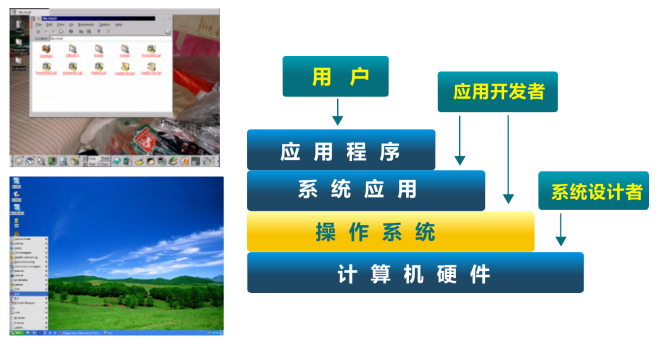
\includegraphics[width=0.5\linewidth]{os-position}
	\caption{承上启下的操作系统}
\end{figure}

\end{frame}


\begin{frame}

\frametitle{操作系统解释}

\begin{columns}

\begin{column}{.6\linewidth}

%\begin{figure}
%	\centering
	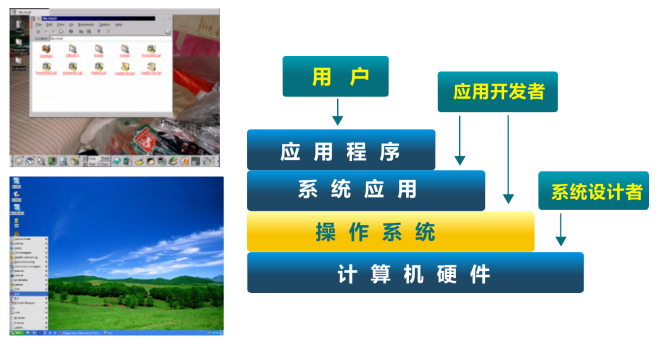
\includegraphics[width=1\linewidth]{os-position}
%	\caption{承上启下的操作系统}

%\end{figure}
\end{column}

\begin{column}{.7\linewidth}
	
\begin{itemize}
\item 没有公认的精确定义 \pause
\item 操作系统是一个控制程序
	\begin{itemize}
	\item 一个系统软件
	\item 控制程序执行过程,防止错误
	\item 执行用户程序,给程序提供服务
	\item 方便用户使用计算机系统
	\end{itemize}
	\pause
	\item 操作系统是一个资源管理程序
	\begin{itemize}
		\item 应用程序与硬件之间的中间层
		\item 管理各种软硬件资源
		\item 提供访问软硬件资源的高效手段
		\item 解决访问冲突,确保公平使用
	\end{itemize}
\end{itemize}

\end{column}

\end{columns}

\end{frame}


%\begin{frame}
%\frametitle{操作系统定义}
%
%\begin{itemize}
%	\item 没有公认的精确定义
%	\item 操作系统是一个资源管理器
%	\begin{itemize}
%		\item 应用程序与硬件之间的中间层
%		\item 管理各种计算机软硬件资源
%		\item 提供访问计算机软硬件资源的高效手段
%		\item 解决资源访问冲突,确保资源公平使用
%	\end{itemize}
%\end{itemize}
%
%\end{frame}
%
%
%\begin{frame}
%	\frametitle{操作系统的位置}
%\begin{figure}
%	\centering
%	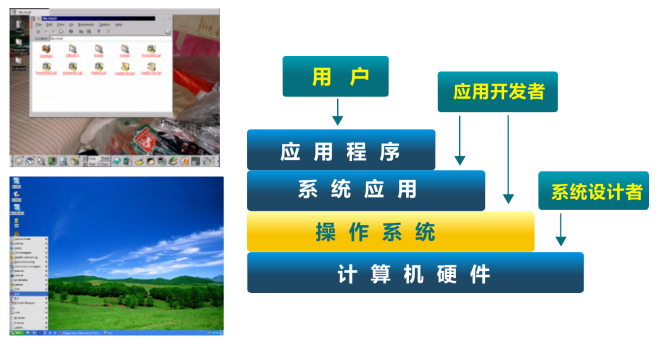
\includegraphics[width=0.8\linewidth]{os-position}
%	\caption{承上启下的操作系统}
%\end{figure}
%\end{frame}

\begin{frame}
	\frametitle{操作系统软件的分类}
		\begin{itemize}
		\item Shell -- 命令行接口
		\item GUI -- 图形用户接口
		\item Kernel--操作系统的内部
	\end{itemize}
	\begin{figure}
		\centering
		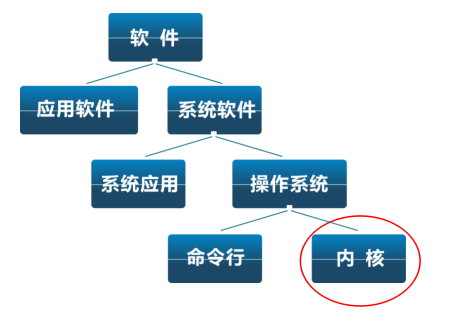
\includegraphics[width=0.6\linewidth]{sort-of-os}
		\caption{操作系统的软件分类}
	\end{figure}
\end{frame}

\begin{frame}
	\frametitle{ucore/rcore教学操作系统内核}
	\begin{figure}
		\centering
		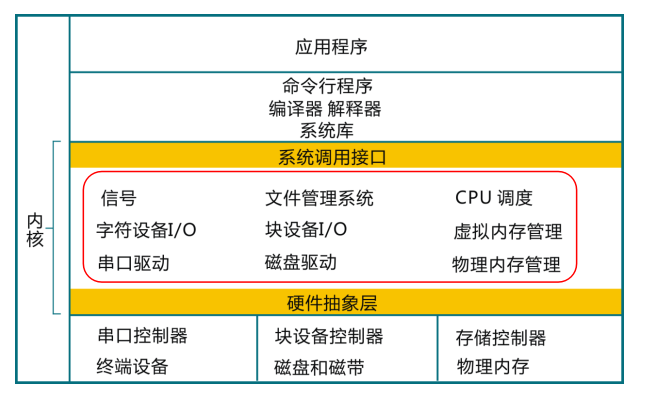
\includegraphics[width=0.8\linewidth]{ucore-arch}
		\caption{ucore/rcore操作系统内核}
	\end{figure}
\end{frame}



\begin{frame}
	\frametitle{操作系统内核的抽象与特征}
	\begin{figure}
	\centering
	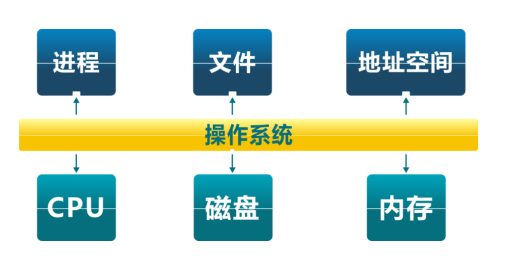
\includegraphics[width=0.5\linewidth]{os-abstract}
	\caption{操作系统抽象}
\end{figure} \pause
	\textbf{操作系统内核的特征}
	\begin{itemize}
		\item 并发:计算机系统中同时存在多个运行程序 \pause
		\item 共享:程序间“同时”访问 互斥共享各种资源 \pause
		\item 虚拟:每个程序"独占"一个完整的计算机 \pause
		\item 异步:服务的完成时间不确定,也可能失败
	\end{itemize}

\end{frame}
%----------------------------------------------------------------------------------------

\end{document}
